\documentclass[12pt]{article}
\usepackage[utf8]{inputenc}
\usepackage[T1]{fontenc}
\usepackage[spanish,es-lcroman]{babel}
\usepackage{amsmath}
\usepackage{amsthm}
\usepackage{bm}
\usepackage{amsfonts}
\usepackage{amssymb}
\usepackage{physics}
\usepackage{tikz}
\usepackage{float}
\usepackage{calc}
\usepackage[autostyle,spanish=mexican]{csquotes}
\usepackage[per-mode=symbol]{siunitx}
\usepackage{textcomp, gensymb}
\usepackage{multicol}
\usepackage{enumitem}
\usepackage{graphicx}
\usepackage{hyperref}
\usepackage{bookmark}
\usepackage{setspace}
\usepackage[left=2.00cm, right=2.00cm, top=2.00cm, 
     bottom=2.00cm]{geometry}
% \usepackage{Estilos/ColoresLatex}
\usepackage{makecell}
% \usepackage{subcaption}
\usepackage[skip=10pt, indent=30pt]{parskip}
% \usepackage{scalerel}
\usepackage{scalerel}[2016-12-29]
% \usepackage{biblatex}
\usepackage{cancel}
\usepackage{caption}
\usepackage{capt-of}
\usepackage[outdir=./Imagenes/]{epstopdf}

\graphicspath{{Imagenes/}}
\DeclareGraphicsExtensions{.png,.jpg,.eps}

\definecolor{ao}{rgb}{0.0, 0.0, 1.0}

\hypersetup{
    colorlinks=true,
    linkcolor=ao,
    filecolor=magenta,      
    urlcolor=ao,
}

\newcommand{\ptilde}[1]{\ensuremath{{#1}^{\prime}}}
\newcommand{\stilde}[1]{\ensuremath{{#1}^{\prime \prime}}}
\newcommand{\ttilde}[1]{\ensuremath{{#1}^{\prime \prime \prime}}}
\newcommand{\ntilde}[2]{\ensuremath{{#1}^{(#2)}}}
\newcommand{\pderivada}[1]{\ensuremath{{#1}^{\prime}}}
\newcommand{\sderivada}[1]{\ensuremath{{#1}^{\prime \prime}}}
\newcommand{\tderivada}[1]{\ensuremath{{#1}^{\prime \prime \prime}}}
\newcommand{\nderivada}[2]{\ensuremath{{#1}^{(#2)}}}

\def\stretchint#1{\vcenter{\hbox{\stretchto[440]{\displaystyle\int}{#1}}}}
\def\scaleint#1{\vcenter{\hbox{\scaleto[3ex]{\displaystyle\int}{#1}}}}
\def\scaleiint#1{\vcenter{\hbox{\scaleto[6ex]{\displaystyle\iint}{#1}}}}
\def\scaleiiint#1{\vcenter{\hbox{\scaleto[6ex]{\displaystyle\iiint}{#1}}}}
\def\scaleoint#1{\vcenter{\hbox{\scaleto[3ex]{\displaystyle\oint}{#1}}}}
\def\bs{\mkern-12mu}

% \newcommand{\textbf}[2]{\textbf{\textcolor{#1}{#2}}}
\sisetup{per-mode=symbol}
\decimalpoint
\sisetup{bracket-numbers = false}
\newlength{\depthofsumsign}
\setlength{\depthofsumsign}{\depthof{$\sum$}}
\newcommand{\nsum}[1][1.4]{% only for \displaystyle
    \mathop{%
        \raisebox
            {-#1\depthofsumsign+1\depthofsumsign}
            {\scalebox
                {#1}
                {$\displaystyle\sum$}%
            }
    }
}

\AtBeginDocument{\RenewCommandCopy\qty\SI}
\ExplSyntaxOn
\msg_redirect_name:nnn { siunitx } { physics-pkg } { none }
\ExplSyntaxOff

\numberwithin{equation}{section}

\linespread{1.25}

\renewcommand{\labelenumii}{\theenumii}
\renewcommand{\theenumii}{\theenumi.\arabic{enumii}.}

\emergencystretch=1em

\title{Completes en eigenfunciones}
\author{M. en C. Gustavo Contreras Mayén}
\date{ }

\begin{document}
\maketitle
\fontsize{14}{14}\selectfont
\spanishdecimal{.}
\tableofcontents
\newpage

%Ref. Arfken (2006) 10.4
\section{Tercera propiedad Operadores autoadjuntos.}
\subsection{Completes de las eigenfunciones.}

La tercera propiedad importante de un operador autoadjunto (Hermitiano) consiste en que \textbf{las eigenfunciones forman un conjunto completo}. Esta completes significa que cualquier función bien portada (al menos en partes pero continua) $F (x)$ se puede aproximar por una serie:
\begin{align}
F (x) = \nsum_{n=0}^{\infty} a_{n} \, \phi_{n} (x) 
\label{eq:ecuacion_10_62}
\end{align}
con cualquier grado de precisión.
\par
Con mayor formalismo, el conjunto $\phi_{n} (x)$ se dice que es \textbf{ao}{completo}, si en el límite el error medio cuadrado se anula:
\begin{align}
\lim_{m \to \infty} \scaleint{6ex}_{\bs a}^{b} \bigg[ F (x) - \nsum_{n=0}^{m} a_{n} \, \phi_{n} (x) \bigg]^{2} \, \sigma (x) \dd{x} = 0
\label{eq:ecuacion_10_63}
\end{align}
Técnicamente, esta es una integral de Lebesgue. No necesariamente el error es nulo en $[a,b]$, pero sólo la integral del error al cuadrado debe ser cero.
\par
La convergencia en la media (ec. \ref{eq:ecuacion_10_63}) debe compararse con la convergencia uniforme. La convergencia uniforme implica la convergencia en la media, pero de manera inversa no se garantiza, la convergencia en la media es menos restrictiva.
\par
En la ecuación (\ref{eq:ecuacion_10_63}) no es válida para funciones continuas en partes, ya que hay un número finito de discontinuidades. Un ejemplo relevante es \textbf{el fenómeno de Gibbs} de las series discontinuas de Fourier, que también ocurre para otras series de funciones propias. En la figura (\ref{fig:figura_fenomeno_Gibss}) se presenta este fenómeno con la función $f (x) = \mbox{sign } (x) \in [-\pi, \pi]$
\begin{figure}
  \centering
  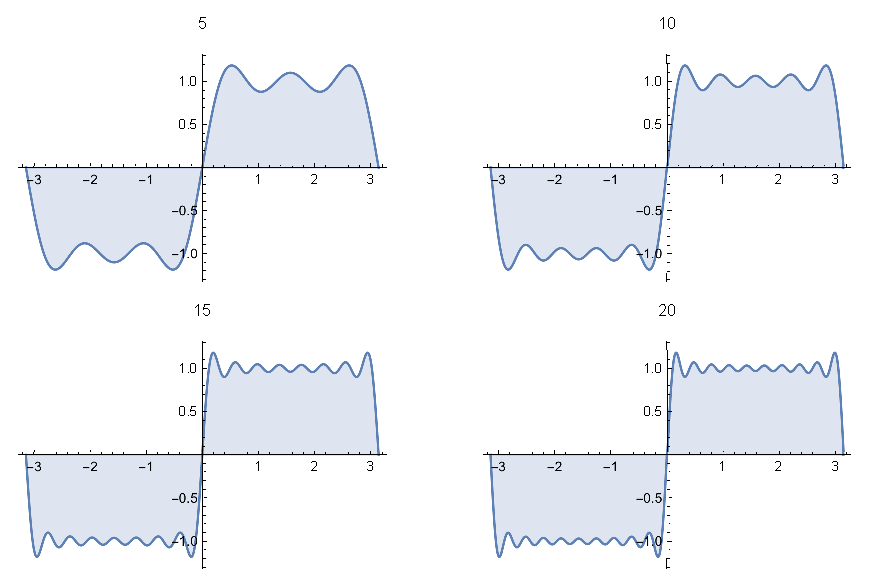
\includegraphics[scale=0.7]{Imagenes/Gibbs_Fourier.eps}
  \caption{El comportamiento oscilante en los extremos es lo que se conoce como fenómeno de Gibss.}
  \label{fig:figura_fenomeno_Gibss}
\end{figure}

En la ecuación (\ref{eq:ecuacion_10_62}) la expansión de los coeficientes $a_{m}$ se determinan mediante:
\begin{align}
a_{m} = \scaleint{6ex}_{\bs a}^{b} F (x) \, \phi_{m}^{*} (x) \, \sigma (x) \dd{x}
\label{eq:ecuacion_10_64}
\end{align}
Que se obtiene al multiplicar la ecuación (\ref{eq:ecuacion_10_62}) por $\phi_{m}^{*} (x) \, \sigma (x)$ y luego se integra. De la ortogonalidad de las eigenfunciones $\phi_{n} (x)$, solo el $m$-ésimo término sobrevive, por lo que la ortogonalidad es importante.
\par
La ecuación (\ref{eq:ecuacion_10_64}) puede compararse con el producto interno de vectores. En ocasiones los coeficientes $a_{m}$ son llamados \textbf{coeficientes generalizados de Fourier}.
\par
Para una función conocida $F (x)$, la ecuación (\ref{eq:ecuacion_10_64}) proporciona los $a_{m}$ como una \textbf{integral definida} que siempre se puede evaluar, ya sea numéricamente si es que no es de manera analítica.
\par
En términos del álgebra lineal, tenemos un espacio lineal, un espacio de funciones. Las funciones linealmente independientes, ortonormales $\phi_{n} (x)$ forman una base de ese espacio (infinito-dimensional).
\par
La ecuación (\ref{eq:ecuacion_10_62}) es un punto que nos dice que las funciones $\phi_{n} (x)$ cubre ese espacio lineal. Con un producto punto definido por la ec. (\ref{eq:ecuacion_10_64}), el espacio lineal que tenemos, se convierte en un \textbf{espacio de Hilbert}.
\par
Por simplicidad, dejando la función de peso $\sigma (x) = 1$, la cerradura en forma de un operador para un conjunto discreto de eigenfunciones $\ket{\phi_{i}}$ es:
\begin{align*}
\setlength{\fboxsep}{3\fboxsep}\boxed{
\nsum_{i} \ket{\varphi_{i}} \bra{\varphi_{i}} =  1}
\end{align*}
Multiplicando la relación de cerradura por $\ket{F}$ obtenemos la expansión de la eigenfunción:
\begin{align*}
\setlength{\fboxsep}{3\fboxsep}\boxed{
\ket{F} = \nsum_{i} \ket{\phi_{i}} \braket{\phi_{i}}{F}}
\end{align*}
con el coeficiente generalizado de Fourier $a_{i} = \braket{\phi_{i}}{F}$. De manera equivalente en una representación coordenada:
\begin{align*}
\setlength{\fboxsep}{3\fboxsep}\boxed{
\nsum_{i} \phi_{i}^{*} (y) \, \phi_{i} (x) = \delta (x - y)}
\end{align*}
Implica que:
\begin{eqnarray*}
\begin{aligned}
F (x) &= \scaleint{6ex} \, F(y) \, \delta (x - y) \, \dd{y} = \nsum_{i} \phi_{i} (x) \, \scaleint{6ex} \, \phi_{i}^{*} (y) \, F(y) \dd{y}
\end{aligned}
\end{eqnarray*}
Sin pruebas, afirmamos que el espectro de un operador lineal $A$ que mapea un espacio de Hilbert $\mathcal{H}$ en sí mismo  puede dividirse en un espectro discreto (o puntual) con eigenvectores de longitud finita.
\par
Un espectro continuo para que la ecuación de eigenvalores $A \, v = \lambda \, v$ con $v$ en $\mathcal{H}$ no tiene una inversa acotada única $(A - \lambda)^{-1}$ en un dominio denso de $\mathcal{H}$. Y un espectro residual donde $(A - \lambda)^{-1}$ está no acotado en un dominio no denso en $\mathcal{H}$.

\subsection{Desigualdad de Bessel.}

Si el conjunto de funciones $\phi_{n} (x)$ \textbf{no forma un conjunto completo},  posiblemente sea por que no se han incluido el número infinito de elementos del conjunto completo, esto nos conduce a la \textbf{desigualdad de Bessel}.
\par
Consideremos primero un caso finito. Sea $\vb{A}$ un vector de $n$ componentes:
\begin{align}
\vb{A} = \vu{e}_{1} \, a_{1} + \vu{e}_{2} \, a_{2} + \ldots + \vu{e}_{n} \, a_{n} 
\label{eq:ecuacion_10_66}
\end{align}
en donde $\vu{e}_{i}$ es un vector unitario y $a_{i}$ es la correspondiente componente (proyección) de $\vb{A}$. Esto es:
\begin{align}
a_{i} = \vb{A} \cdot \vu{e}_{i}
\label{eq:ecuacion_10_67}
\end{align}
Entonces:
\begin{align}
\left( \vb{A} - \nsum_{i} \vu{e}_{i} \, a_{i} \right)^{2} \geq 0
\label{eq:ecuacion_10_68}
\end{align}
Si sumamos todos los $n$ componentes, evidentemente la suma se iguala a $\vb{A}$ por la ecuación (\ref{eq:ecuacion_10_66}) y la igualdad es consistente. Pero cuando la suma no incluye a todos los $n$ componentes, resulta la desigualdad.
\par
Expandiendo la ecuación (\ref{eq:ecuacion_10_68}) y eligiendo los vectores unitarios para que satisfagan la relación de ortogonalidad:
\begin{align}
\vu{e}_{i} \cdot \vu{e}_{j} = \delta_{ij}
\label{eq:ecuacion_10_69}
\end{align}
Tenemos que:
\begin{align}
\vb{A}^{2} \geq \nsum_{i} a_{i}^{2}
\label{eq:ecuacion_10_70}
\end{align}
Que es \underline{\textbf{la desigualdad de Bessel}}.
\par
En el caso continuo para funciones reales debemos de considerar la integral:
\begin{align}
\scaleint{7ex}_{\bs a}^{b} \left[ f (x) - \nsum_{i} a_{i} \, \phi_{i} (x) \right]^{2} \, \sigma (x) \dd{x} \geq 0
\label{eq:ecuacion_10_71}
\end{align}
que es el análogo continuo de la ecuación (\ref{eq:ecuacion_10_68}), haciendo $n \to \infty$ y reemplazando la suma por la integración. Nuevamente, con el factor de peso $\sigma (x) > 0 $, el integrando es no negativo.
\par
La integral se anula por la ecuación (\ref{eq:ecuacion_10_62}) si tenemos un conjunto completo.  De otra forma, es positiva. Desarrollando el término al cuadrado obtenemos:
\begin{equation}
\begin{aligned}
\scaleint{6ex}_{\bs a}^{b} \big[ f (x) \big]^{2} \, \sigma (x) \dd{x} &- 2 \nsum_{i} a_{i} \, \scaleint{6ex}_{\bs a}^{b} f (x) \, \phi (x) \, \sigma (x) \dd{x} + \\[0.5em]
&+ \nsum_{i} a_{i}^{2} \geq 0
\end{aligned}
\label{eq:ecuacion_10_72}
\end{equation}
Usando la ecuación (\ref{eq:ecuacion_10_64}), tenemos:
\begin{equation}
\scaleint{6ex}_{\bs a}^{b} \big[ f (x) \big]^{2} \, \sigma (x) \dd{x} \geq \nsum_{i} a_{i}^{2}
\label{eq:ecuacion_10_73}
\end{equation}
De aquí que la suma de los cuadrados de la expansión de los coeficientes $a_{i}$ es menor o igual que la integral ponderada de $[f (x)]^{2}$,  la igualdad se mantiene si y sólo si,  la expansión es exacta,  esto ocurre si el conjunto de soluciones $\phi_{n} (x)$ es un conjunto completo.
\par
Cuando se considera que las eigenfunciones que forman conjuntos completos (como los polinomios de Legendre), la ec. (\ref{eq:ecuacion_10_73}) con el signo igual que se mantiene se llamará \textbf{relación de Parseval}.
\par
La desigualdad de Bessel tiene distintos usos, incluida la prueba de convergencia para las series de Fourier.

\subsection{Desigualdad de Schwarz.}

La desigualdad de Schwarz de uso frecuente es similar a la desigualdad de Bessel. Consideremos la ecuación cuadrática con la incógnita $x$:
\begin{align}
\nsum_{i=1}^{n} (a_{i} \, x + b_{i})^{2} = \nsum_{i=1}^{n} a_{i}^{2} \left( x + \dfrac{b_{i}}{a_{i}} \right)^{2} = 0
\label{eq:ecuacion_10_74}
\end{align}
con $a_{i}$, $b_{i}$ reales. Se presentan los dos siguientes casos en el cociente:
\begin{enumerate}
\item Si $b_{i}/a_{i}$ es la constante $c$, independiente del índice $i$, la solución es $x= - c$.
\item Si $b_{i}/a_{i}$ no es constante en $i$, todos los términos no se anulan simultáneamente para un $x$ real, por lo que la solución debe de ser compleja.
\end{enumerate}
Expandiendo, tenemos que:
\begin{align}
x^{2} \, \nsum_{i}^{n} a_{i}^{2} + 2 \, x \, \nsum_{i}^{n} a_{i} \, b_{i} + \nsum_{i}^{n} b_{i}^{2} = 0
\label{eq:ecuacion_10_75}
\end{align}
Como $x$ es complejo (o = $-b_{i}/a_{i}$), la fórmula cuadrática para $x$ conduce a:
\begin{align}
\left( \nsum_{i=1}^{n} a_{i} \, b_{i} \right)^{2} \leq \left( \nsum_{i=1}^{n} a_{i}^{2} \right) \, \left( \nsum_{i=1}^{n} b_{i}^{2} \right)
\label{eq:ecuacion_10_76}
\end{align}
la igualdad se mantiene cuando $b_{i}/a_{i}$ es una constante independiente de $i$.
\par
En el caso discreto, nuevamente en términos de vectores, tenemos que:
\begin{align}
( \vb{a} \cdot \vb{b} )^{2} =  a^{2} \, b^{2} \, \cos^{2} \theta \leq a^{2} \, b^{2}
\label{eq:ecuacion_10_77}
\end{align}
donde $\theta$ es el ángulo entre $\vb{a}$ y $\vb{b}$.

La desigualdad de Schwarz para funciones complejas tiene la expresión:
\begin{align}
&\abs{ \scaleint{6ex}_{\bs a}^{b} f^{*} (x) \, g (x) \dd{x} }^{2} \leq \scaleint{6ex}_{\bs a}^{b} f^{*} (x) \, f (x) \dd{x} \scaleint{6ex}_{\bs a}^{b} g^{*} (x) \, g (x) \dd{x}
\label{eq:ecuacion_10_78}
\end{align}
La desigualdad se mantiene si y sólo si:
\begin{align*}
g (x) = \alpha \, f (x)
\end{align*}
siendo $\alpha$ una constante. Para probar esta forma de la función de la desigualdad de Schwarz, consideremos la función compleja:
\begin{align*}
\psi (x) = f(x) + \lambda \, g (x)
\end{align*}
con $\lambda$ una constante compleja, donde las funciones $f (x)$ y $g (x)$ son cualesquiera dos funciones de cuadrado integrable (para las cuales, las integrales del lado derecho existen). Multiplicando por el conjugado complejo y luego integrando, tenemos:
\begin{align}
\begin{aligned}
\scaleint{6ex}_{\bs a}^{b} \psi^{*} \, \psi \dd{x} &\equiv \scaleint{6ex}_{\bs a}^{b} f^{*} \, f \dd{x} + \lambda \, \int_{a}^{b} f^{*} \, g \dd{x} + \lambda^{*} \, \scaleint{6ex}_{\bs a}^{b} g^{*} \, f \dd{x} + \\
&+ \lambda \, \lambda^{*} \, \scaleint{6ex}_{\bs a}^{b} g^{*} \, g \, \dd{x}  \geq 0
\end{aligned}
\label{eq:ecuacion_10_79}
\end{align}
Interpretando la desigualdad:
\begin{enumerate}
\item El $\geq 0$ aparece ya que $\psi^{*} \, \psi$ es no negativo.
\item El signo igual $(=)$ se mantiene sólo si $\psi (x)$ es idéntico a cero.
\end{enumerate}
Nótese que $\lambda$ y $\lambda^{*}$ son linealmente independientes,  diferenciamos con respecto a uno de ellos,  e igualamos la derivada a cero para minimizar $\displaystyle \int_{a}^{b} \psi^{*} \, \psi \dd{x}$:
\begin{align*}
\pdv{\lambda^{*}} \scaleint{6ex}_{\bs a}^{b} \psi^{*} \, \psi \dd{x} = \scaleint{6ex}_{\bs a}^{b} g^{*} \, f \dd{x}  + \lambda \scaleint{6ex}_{\bs a}^{b} g^{*} g \dd{x} = 0
\end{align*}
Que nos lleva a:
\begin{align}
\lambda = - \, \dfrac{\displaystyle \scaleint{6ex}_{\bs a}^{b} g^{*} \, f \dd{x}}{\displaystyle \scaleint{6ex}_{\bs a}^{b} g^{*} \, g \dd{x}}
\label{eq:ecuacion_10_80a}
\end{align}
Tomando el conjugado complejo:
\begin{align}
\lambda^{*} = - \dfrac{\displaystyle \scaleint{6ex}_{\bs a}^{b} f^{*} \, g \dd{x}}{\displaystyle \scaleint{6ex}_{\bs a}^{b} g^{*} \, g \dd{x}}
\label{eq:ecuacion_80b}
\end{align}
Sustituyendo esos valores de $\lambda$ y $\lambda^{*}$ en la ecuación (\ref{eq:ecuacion_10_79}),  obtenemos la ecuación (\ref{eq:ecuacion_10_78}), \underline{\textbf{la desigualdad de Schwarz}}.

\textbf{Ejemplo de la mecánica cuántica: } En mecánica cuántica las funciones $f (x)$ y $g (x)$ podrían representar un estado o una configuración de un sistema físico, es decir, una combinación lineal de funciones de onda. Entonces la desigualdad e Schwarz garantiza que el producto punto $\displaystyle \int_{a}^{b} f^{*} (x) \, g(x) \, \dd{x}$ existe.
\par
En algunos textos, la desigualdad de Schwarz es un paso para llegar al principio de incertidumbre de Heisenberg.
\par
La notación de las funciones de las ecuaciones (\ref{eq:ecuacion_10_78}) y (\ref{eq:ecuacion_10_79}) es a veces incómoda;  en mecánica cuántica es común utilizar la notación de Dirac. Con esta notación, se simplifica tanto el rango de integración $(a, b)$, como la función de peso $\sigma (x) \geq 0$. 
\par
La desigualdad de Schwarz ahora se representa:
\begin{align}
\abs{\braket{f}{g}}^{2} \leq \braket{f}{f} \, \braket{g}{g}
\label{eq:ecuacion_10_78a}
\end{align}
Si $g (x)$ es una eigenfunción normalizada, $\phi_{i} (x)$, la ecuación (\ref{eq:ecuacion_10_78}) nos lleva a (donde $\sigma (x) = 1$):
\begin{align}
a_{i}^{*} \, a_{i} \leq \scaleint{6ex}_{\bs a}^{b} f^{*} (x) \, f (x) \dd{x} 
\label{eq:ecuacion_10_81}
\end{align}
Que es un resultado que se sigue de la ecuación (\ref{eq:ecuacion_10_73}).

% %Ref. Arfken (1981) pág. 514

\section{Representación con la delta de Dirac.}
\subsection{Eigenfunciones y la delta de Dirac.}

El conjunto ortonormal de eigenfunciones $\phi_{n} (x)$ proporciona otra representación interesante de la función delta de Dirac. Consideremos la suma:
\begin{align}
K (x, t) = K (t, x) = \nsum_{n=0}^{\infty} \phi_{n} (x) \, \phi_{n} (t)
\label{eq:ecuacion_09_80}
\end{align}
Por conveniencia, se supone que $\phi_{n} (x)$ se ha definido para incluir $[\sigma (x)]^{1/2}$ si $\sigma (x) \neq 1$. Esta serie en la ec. (\ref{eq:ecuacion_09_80}) de hecho no es convergente uniformemente,  pero puede utilizarse como parte de un integrando en donde la integración subsecuente la convierta en convergente.
\par
Supongamos ahora que se forma la integral:
\begin{align*}
\scaleint{6ex} F (t) \, K (x, t) \dd{t}
\end{align*}
en donde se considera que $F (t)$ se puede desarrollar en serie de eigenfunciones $\phi_{p} (t)$. Se tiene que:
\begin{eqnarray}
\begin{aligned}[b]
\scaleint{6ex} &F (t) \, K (x, t) \dd{t} = \scaleint{6ex} \nsum_{p=0}^{\infty} a_{p} \, \phi_{p} (t) \, \nsum_{n=0}^{\infty} \phi_{n} (x) \, \phi_{n} (t) \dd{t} = \\[0.5em] 
&= \nsum_{p=0}^{\infty} a_{p} \, \phi_{p} (x) =  F (x)
\end{aligned}
\label{eq:ecuacion_09_81}
\end{eqnarray}
en que los productos opuestos $\phi_{p} \, \phi_{n} \, (n \neq p)$ desaparecen por ortogonalidad.
\par
Al tomar en cuenta la definición de la función delta de Dirac, el resultado de la ec. (\ref{eq:ecuacion_09_81}) significa que:
\begin{align}
K (x, t) = \delta (x - t) = \nsum_{n=0}^{\infty} \phi_{n} (x) \, \phi_{n} (t)
\label{eq:ecuacion_09_82}
\end{align}
Es fácil demostrar que:
\begin{align}
\scaleint{6ex} K (x, t) \dd{t} = 1
\label{eq:ecuacion_09_83}
\end{align}
permitiendo que $F (t) = \phi_{0}$, una constante.
La confirmación del comportamiento en $x = t$ se encuentra al utilizar la desigualdad de Bessel. Se tiene que:
\begin{align}
K (t, t) = \nsum_{n=0}^{\infty} \big[ \phi_{n} (t) \big]^{2}
\label{eq:ecuacion_09_84}
\end{align}
Usando la ec. (\ref{eq:ecuacion_10_73}), se obtiene:
\begin{align}
\scaleint{6ex} \big[ K (t, t) \big]^{2} \dd{t} = \nsum_{n=0}^{\infty} a_{n}^{2} = \nsum_{n=0}^{\infty} 1 = \infty
\label{eq:ecuacion_09_85}
\end{align}
En consecuencia, $K(x, t)$ diverge en $x = t$, tal como era de esperarse.

% %Ref. Arfken 10.5 (2006)
\section{Función de Green.}
\subsection{Expansión en eigenfunciones.}

Una serie algo similar a la representada por $K (x, t)$ - que es a la vez $\delta (x - t)$ -  resulta cuando se desarrolla la función de Green en eigenfunciones de la ecuación homogénea correspondiente.
\par
En la ecuación de Helmholtz no homogénea se tiene que:
\begin{align}
\setlength{\fboxsep}{3\fboxsep}\boxed{
\laplacian \psi (\vb{r}) + k^{2} \, \psi (\vb{r}) = - \rho (\vb{r})
\label{eq:ecuacion_10_82}}
\end{align}
La ecuación de Helmholtz homogénea se satisface con sus eigenfunciones ortonormales $\varphi_{n}$:
\begin{align}
\laplacian \varphi_{n} (\vb{r}) + k_{n}^{2} \, \varphi_{n} (\vb{r}) = 0
\label{eq:ecuacion_10_83}
\end{align} 
La función de Green $G (\vb{r}_{1}, \vb{r}_{2})$ satisface la ecuación de la fuente en el punto:
\begin{align}
\setlength{\fboxsep}{3\fboxsep}\boxed{
\laplacian G (\vb{r}_{1}, \vb{r}_{2}) + k^{2} \, G (\vb{r}_{1}, \vb{r}_{2}) = - \delta (\vb{r}_{1}- \vb{r}_{2})}
\label{eq:ecuacion_10_84}
\end{align}
con las condiciones de frontera impuestas en las soluciones de la ecuación homogénea.
\par
Dado que $G$ es real,  se desarrolla la función de Green en la forma de serie de funciones propias de la ecuación homogénea, ec. (\ref{eq:ecuacion_10_83}), es decir:
\begin{align}
G (\vb{r}_{1}, \vb{r}_{2}) = \nsum_{n=0}^{\infty} a_{n} (\vb{r}_{2}) \, \varphi_{n} (\vb{r}_{1})
\label{eq:ecuacion_10_85}
\end{align}
Que al sustituir en la ec. (\ref{eq:ecuacion_10_84}), se obtiene:
\begin{align}
\begin{aligned}[b]
- \nsum_{n=0}^{\infty} &a_{n} (\vb{r}_{2}) k_{n}^{2} \varphi_{n} (\vb{r}_{1}) + k^{2} \nsum_{n=0}^{\infty} a_{n} (\vb{r}_{2}) \varphi_{n} (\vb{r}_{1}) = - \nsum_{n=0}^{\infty} \varphi_{n} (\vb{r}_{1}) \, \varphi_{n} (\vb{r}_{2})
\end{aligned}
\label{eq:ecuacion_10_86}
\end{align}
Aquí, la $\delta (\vb{r}_{1} - \vb{r}_{2})$ se ha sustituido por su desarrollo de eigenfunción.
\par
Cuando se utiliza la ortogonalidad de $\varphi_{n} (\vb{r}_{1})$ para aislar $a_{n}$, nos lleva a:
\begin{align*}
&\nsum_{m=0}^{\infty} a_{m} (\vb{r}_{2}) \, \big( k_{n}^{2} - k_{m}^{2} \big) \, \scaleint{6ex} \varphi_{n} (\vb{r}_{1}) \, \varphi_{m} (\vb{r}_{1}) \dd[3]{r_{1}} = \\[0.5em]
&- \nsum_{n=0}^{\infty} \varphi_{m} (\vb{r}_{2})  \, \scaleint{6ex} \varphi_{n} (\vb{r}_{1}) \, \varphi_{m} (\vb{r}_{1}) \dd[3]{r_{1}}    
\end{align*} 
De manera equivalente:
\begin{align*}
a_{n} (\vb{r}_{2}) \, \big( k^{2} - k_{n}^{2} \big) = - \varphi_{n} (\vb{r}_{2})
\end{align*}
Que al sustituir en la ec. (\ref{eq:ecuacion_10_85}), la función de Green se transforma en:
\begin{align}
\setlength{\fboxsep}{3\fboxsep}\boxed{
G (\vb{r}_{1}, \vb{r}_{2}) = \nsum_{n=0}^{\infty} \dfrac{\varphi_{n} (\vb{r}_{1}) \, \varphi_{n} (\vb{r}_{2})}{k_{n}^{2} - k^{2}}}
\label{eq:ecuacion_10_87}
\end{align}
que es un desarrollo bilineal, simétrico con respecto a $\vb{r}_{1}$ y $\vb{r}_{2}$ como era de esperarse. Finalmente, $\psi (\vb{r}_{1})$, la solución deseada para la ecuación no homogénea está dada por:
\begin{align}
\setlength{\fboxsep}{3\fboxsep}\boxed{
\psi (\vb{r}_{1}) = \scaleint{6ex} G (\vb{r}_{1}, \vb{r}_{2}) \, \rho (\vb{r}_{2}) \dd{\tau_{2}}}
\label{eq:ecuacion_10_88}
\end{align}

Si se generaliza la ecuación diferencial no homogénea a:
\begin{align}
\mathcal{L} \psi + \lambda \, \psi = - \rho
\label{eq:ecuacion_10_89}
\end{align}
en donde $\mathcal{L}$ es el operador Hermitiano. Se tiene que:
\begin{align}
G (\vb{r}_{1}, \vb{r}_{2}) = \nsum_{n=0}^{\infty} \dfrac{\varphi_{n} (\vb{r}_{1}) \, \varphi_{n} (\vb{r}_{2})}{\lambda_{n} - \lambda}
\label{eq:ecuacion_10_90}
\end{align}
En donde $\lambda_{n}$ es el n-ésimo eigenvalor de $\varphi_{n}$,  la eigenfunción normal correspondiente a la ED homogénea:
\begin{align}
\mathcal{L} \, \psi + \lambda \, \psi = 0
\label{eq:ecuacion_10_91}
\end{align}
La expansión en eigenfunciones de la función de Green en la ec. (\ref{eq:ecuacion_10_90}) hace explícita la propiedad de simetría:
\begin{align*}
G (\vb{r}_{1}, \vb{r}_{2}) = G (\vb{r}_{2}, \vb{r}_{1})
\end{align*}
y es útil cuando se compara con soluciones obtenidas por otros medios.

\section{Ejercicios.}
\subsection{Ejercicios a cuenta.}

\begin{enumerate}
%Ref. Arfken 10.4.4
\item \textbf{Ejercicio.} En lugar de la expansión de una función $F(x)$ dada por:
\begin{align*}
F (x) = \nsum_{n=0}^{\infty} a_{n} \, \varphi_{n} (x)
\end{align*}
con los coeficientes:
\begin{align*}
a_{n} = \scaleint{6ex}_{\bs a}^{b} F(x) \, \varphi_{n} (x) \, \omega (x) \dd{x}
\end{align*}
Considera la aproximación por una serie \textbf{finita}:
\begin{align*}
F (x) \approx \nsum_{n=0}^{m} c_{n} \, \varphi_{n} (x)
\end{align*}
Demuestra que el cuadrado del error medio:
\begin{align*}
\scaleint{6ex}_{\bs a}^{b} \bigg[ F(x) - \nsum_{n=0}^{m} c_{n} \, \varphi_{n} (x) \bigg]^{2} \, \omega (x) \dd{x}
\end{align*}
se minimiza cuando $c_{n} = a_{n}$.
\par
\noindent
\textbf{Nota: } Los valores de los coeficientes son independientes del número de términos en la serie finita. Esta independencia es una consecuencia de la ortogonalidad y no sería válida para un ajuste por mínimos cuadrados utilizando potencias de $x$.
%Ref. Arfken 10.4.7
\item \textbf{Ejercicio.} Recupera la desigualdad de Schwarz de la siguiente identidad:
\begin{align*}
&\bigg[ \scaleint{6ex}_{\bs a}^{b} f(x) \, g(x) \dd{x} \bigg
]^{2} {=} \scaleint{6ex}_{\bs a}^{b} \big[ f(x) \big
]^{2} \dd{x} \, \scaleint{6ex}_{\bs a}^{b} \big[ g(x) \big
]^{2} \dd{x} + \\[0.5em]
&- \dfrac{1}{2} \, \scaleint{6ex}_{\bs a}^{b} \, \scaleint{6ex}_{\bs a}^{b} \bigg[ f(x) \, g(y) - f(y) \, g(x) \bigg
]^{2} \dd{x} \dd{y}
\end{align*}
\textbf{Nota:} Cuida el signo de la expresión, recuerda que al cortar el renglón, se deja el signo $+$, en el siguiente renglón se tiene el signo $-$, por lo que el segundo término está restando el producto del primer término.
\end{enumerate}


\end{document}